\documentclass[a4paper,10pt]{article}
\usepackage[margin=2.5cm, nohead]{geometry}
\usepackage{palatino, url, multicol}
\usepackage{hyperref}
\usepackage{graphicx}
\usepackage{float}
\usepackage{verbatim}
\usepackage[all]{xy}
\usepackage[english]{babel}
\usepackage{cite}


\begin{document}

\begin{center}
\thispagestyle{empty}


\vspace{2.5cm}

% [CHANGE] The title of your thesis. If your thesis has a subtitle, then this
% should appear right below the main title, in a smaller font.
\hrulefill\\
\begin{Huge}
Bachelor project: Midterm report\\
\end{Huge}
\vspace{0.2cm}
\begin{Large} 
Combining Robocup Rescue and Xabsl\\
\end{Large}
\hrulefill\\
\vspace{0.5cm}

\includegraphics[width=\textwidth]{uva.jpg}
\vspace{0.5cm}

% [CHANGE] Your full name. In case of multiple names, you can include their
% initials as well, e.g. "Jan G.J. van der Wegge".
{
\Large
Maarten P. de Waard\\\vspace{0.2cm}
% [CHANGE] Your student ID, as this has been assigned to you by the UvA
% administration.
\textit{5894883}
}

\vspace{1.5cm}

% [DO NOT CHANGE]
Bachelor thesis\\
% [CHANGE] Whether your Bachelor thesis is 6 ECTS (regular) or 9 ECTS (Honours
% programme).
Credits: 6 EC

\vspace{0.5cm}

% [DO NOT CHANGE] The name of the educational programme.
Bsc. Artificial Intelligence

\vspace{0.25cm}

% [DO NOT CHANGE] The addess of the educational programme.
University of Amsterdam\\
Faculty of Science\\
Science Park 904\\
1098 XH Amsterdam

\vspace{2cm}

\emph{Supervisor}\\
% [CHANGE] The name of your supervisor. Include the titles of your supervisor,
% as well as the initials for *all* of his/her first names.
dr. A. Visser 

\vspace{0.25cm}

% [CHANGE] The address of the institute at which your supervisor is working.
% Be sure to include (1) institute (is appropriate), (2) faculty (if
% appropriate), (3) organisation name, (4) organisation address (2 lines).
Informatics Institute\\
Faculty of Science\\
University of Amsterdam\\
Science Park 904\\
1098 XH Amsterdam\\

\vspace{1.5cm}

% [CHANGE] The date at which you will finalize and submit your thesis.
June 26th, 2012

\end{center}
\newpage


\begin{abstract}
When done, this will become the abstract
\end{abstract}

\begin{multicols}{2}
\section{Introduction}
The research will be focussing on combining the \textit{Extensible Agent
Behavior Specification Language} (XABSL) with the current RoboCup Rescue code, used
by Arnoud Visser, in the RoboCup Rescue missions. 

There are currenty different solutions on how to control several robots in a
virtual rescue operation, to find as many victims as possible. Sophisticated
methods have been constructed to control the robots as efficiently as possible.
Some of these, make use of several `behaviors', which can be activated by a
person controlling a robot, or autonomously. For example, a behavior could be a
module that makes the robot navigate to a specified point on the map.

An improvement that can still be made in these behavior controlled robots, is in 
the specification of which behavior should be selected in a certain situation. This can be done by creating
behavior-controlled robots, that can autonomously select the best behavior to
activate on a certain moment.

This research will make use of XABSL, a behavior specification language, which
makes it possible to separate the specification of a behavior, from the implementation.
I will prove high efficiency of this method,
by comparing the results of missions done by different solutions, with
mine. 

Results in the RoboCup Rescue missions are counted by how many victims
are found on the map, so improvement can be shown by finding more victims using
the results of this research.

Currently, not many behavior-controlled exploration algorithms exist. The
closest to this is finding a path on challenging terrain. 
\cite{seraji2002behavior} . Eventually, this research will result in a method to
easily adjust and improve the exploration behavior of the RoboCup Rescue code.


\section{RoboCup Rescue}
\subsection{Description}
The first of the two projects is the program for RoboCup Rescue, called
UsarCommander\footnote{Available at
http://www.jointrescueforces.eu/wiki/tiki-index.php}, originally developed by Bayu Slamet, and extended by Arnoud
Visser and many others. This program takes care of connecting to UsarSim and
makes the user able to easily get sensor data from the robots in it. It is also
possible to control the robots with many types of behavior, or by hand, clicking
arrows on the interface that comes with it.

Over time, the system has been expanded with many subprojects, for example one
implementing a SLAM
(Simultaneous Localisation And Mapping) algorithm, to make an accurate map from
the sensor data of several robots.\cite{slamet2006manifoldslam} All the information used and produced by
these subprojects can be accessed by other subprojects, resulting in an ideal
environment for creating new robot-controlling applications.

\subsection{Motivation to use it}
The main reason to use this program, in stead of any other, to interface my
software with USARSim is that it has so many features. The presence of many
subprojects in the code, makes it possible to make a very efficient autonomous
exploration algorithm using the data available. Without using UsarCommander all
the needed software should be taken from somewhere else, or implemented solely
for this purpose.

Other software for this purpose is available to, but since this is a bachelor
thesis on the University of Amsterdam, and this is the software used by it in
the RoboCup, this is the logical choice.

\section{XABSL}
`XABSL' is a very simple language to descripbe behaviors for autonomous agents
based on hierarchical finite state machines \cite{loetzsch2003xabsl}. It is the
software that has been used by the German robotic soccer team to specify their
robots' behavior. The team won in 2008.

\begin{figure*}
    \centering
        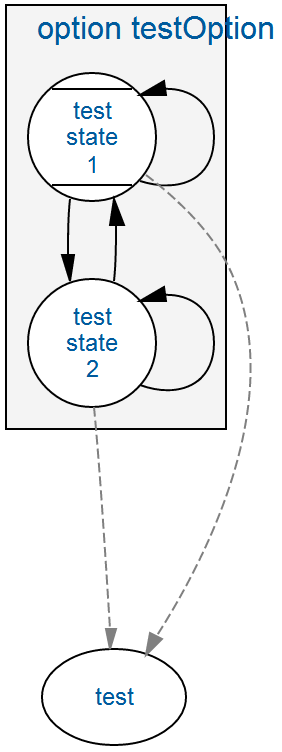
\includegraphics[width=.2\textwidth]{simpleFsm.png}
    \label{fig:simpleFsm}
    \caption{An example of a figure generated by a XABSL tool, from XABSL code.}
\end{figure*}

XABSL makes use of four components: Agents, Options, states and Basic behavior.
The following subsections will explain what these are, and how they can be used.

\subsection{Agents}
An XABSL agent is a rooted acyclic graph, containing all the behaviors for one
agent. In this research, one agent will equal one robot. 



\begin{itemize}
\item \emph{Agents:} A rooted acyclic graph, containing all the behaviors for one
agent. Several of these agents can be created, all having their own graph and
thus their own behavior.
\item \emph{Options:} Complex agent behavior. Each option is on itself a finite
state machine, containing several states.
\item \emph{States:} `Actions' that can be either active or inactive. At least
one state is always active. Each option has an initial state, being the first
state to be active. States are connected with each other by decision trees,
deciding what state or option is activated next.
\item \emph{Basic behavior:} At every leaf of an option (so, every state with no
other states to reference to) a basic behavior is activated. This is a small
piece of C++ code, that influences actions of the agent. 
\end{itemize}



\subsubsection{Motivation to use it}
Using FSM's for behavior is an easily comprehensible method to specify behavior.
The advantages of XABSL are that tools are delivered to make a hierarchy
documentation for your website (or anything else). For example, the FSM in
figure \ref{fig:simpleFsm} is automatically generated from XABSL code.

Using this representation, tweaking the behavior should become an easier task
resulting in better results for autonomous exploration.

% TODO
This section will be expanded with the following: 

\section{Approach}
\begin{comment}
This section will contain my approach
\end{comment}

\subsection{Interfacing both programs}
Since the UsarCommander is written in Visual Basic, and the basic behaviors of
XABSL are written in C++, a bridge should be made. This is done by creating a
Dynamic Link Library (DLL). This DLL contains the needed functions of the C++
program, making them accessible for Visual Basic. The bridge works both ways, so
Visual Basic can offer output symbols to the XABSL Engine, while the engine can
offer input symbols to the agent.

\subsection{Creating a succesful hierarchy}
This section will tell about the FSM hierarchy I will make for autonomous
exploration


\section{Results}
This section will contain results, hopefully in the form of explored maps, numbers of victims found, etc.

\section{Conclusion}

\end{multicols}{2}
\bibliography{bib}{}
\bibliographystyle{plain}
\end{document}

